\chapter{Background and Related Work}
\label{chap:background}

This chapter provides the theoretical and practical background needed to understand the design decisions we make later in the thesis. We start by looking at closed-loop payment systems, which is the category our system falls into, and then move on to the architectural patterns that deal with offline operation and distributed data. We also review the existing commercial solutions for festival payments and discuss the academic literature on conflict resolution in distributed systems. The goal is to give the reader enough context to understand why we made the choices we did, and what alternatives we considered along the way.

\section{Closed-Loop Payment Systems}
\label{sec:closed-loop}

Before going into the technical details, it is worth clarifying what we mean by a closed-loop payment system, since this concept is at the core of our architecture. In the payment industry, there are basically two types of systems: open-loop and closed-loop. An open-loop system is what most people use every day without thinking about it. When you pay with a Visa or Mastercard, the transaction goes through a network of banks, card schemes, and processors that connect merchants to customers across the entire world. The money flows through multiple intermediaries, each taking a small fee, and the whole thing relies on a global infrastructure that has been built over decades.

A closed-loop system is fundamentally different. As described by SDK.finance~\cite{SDKFinance2024}, ``closed-loop payment systems are financial arrangements that confine transactions to a specific network or ecosystem.'' In a closed-loop, the issuer and the acquirer are the same entity, which means a single operator controls the entire flow of money within a defined perimeter. Think of it like this: you load credits into the system, you spend those credits at authorized points, and whatever you did not spend, you can get back as a refund. The money never leaves the operator's ecosystem during the transaction itself. The operator has full control over the rules, the fees, the authorization logic, and most importantly for our use case, the infrastructure.

There are several reasons why closed-loop systems are so attractive for festival environments, and the network situation is just one of them. The first and most obvious reason is the connectivity problem we discussed in Chapter~\ref{chap:introduction}. A festival is already a place where the network is going to have a bad time, so depending on external payment networks like Visa or Mastercard that need to reach authorization servers on the other side of the world is just asking for trouble. With a closed-loop system, all the authorization logic lives inside the operator's own infrastructure, so when the network has issues the system only needs to talk to itself.

The second reason is fees. Open-loop payment processing is not cheap. Every time someone pays with a credit or debit card, the merchant pays an interchange fee to the card issuer, a scheme fee to the card network, and a processing fee to the payment processor. For a small transaction like buying a beer at a festival, these fees can eat up a significant percentage of the sale. In a closed-loop system, the operator cuts out all these intermediaries. There is no interchange fee, no scheme fee, and no processor taking a cut of every transaction. The only point where external fees apply is when money enters the system through a top-up, which involves Stripe or another payment provider, but even then, almoast always these topup fees are lower due to negotiatiosn with the payment provider (that is most likely a strategic partner). Once the money is inside the closed loop, every subsequent transaction is free for the operator. For a festival processing tens of thousands of small transactions per day, this adds up to serious savings.

The third reason is perhaps the most interesting one, and it has to do with regulation. In the European Union, handling electronic money is a regulated activity that requires an e-money license under the Electronic Money Directive (EMD2)~\cite{EMD2009}. Getting an e-money license is an expensive and time-consuming process that involves capital requirements, compliance obligations, and ongoing regulatory oversight. However, many festival payment systems operate in something of a regulatory gray area by using tokens or credits instead of displaying actual currency values. The idea is that when an attendee tops up their wristband or app, they are not depositing money into an electronic wallet in the regulatory sense. Instead, they are purchasing prepaid tokens that can be redeemed at participating vendors within the festival. This distinction matters because prepaid instruments issued for use within a limited network of service providers can fall under an exemption in the Payment Services Directive (PSD2)~\cite{PSD2015}, specifically the limited network exclusion. Under this exemption, if the payment instrument can only be used to acquire goods or services within a limited network of providers (like the vendors inside a festival), the operator may not need a full e-money or payment institution license. This is also why many festival systems show balances in ``tokens'' or ``credits'' rather than in euros or dollars. Displaying the balance as ``50 tokens'' instead of ``50 EUR'' reinforces the narrative that these are not electronic money but rather prepaid vouchers for a specific set of services. Of course, this is a simplification and the legal situation varies by jurisdiction. Some regulators have taken a stricter view, and operators who process large volumes may still need to register or obtain a limited license. But the point is that the closed-loop, token-based model gives festival operators a much simpler regulatory path compared to running a full open-loop payment service.

The fourth reason is control. In a closed-loop system, the festival operator decides everything: transaction limits, refund policies, spending restrictions, which vendors are authorized, and how the settlement process works. There is no card scheme telling you what you can and cannot do. This level of control is particularly valuable for events where the operator needs to manage the entire economy, from how much people can top up to how refunds are handled after the festival ends. And the most important reason, of course, taking a percentage cut out of all the transactions inside the event without having to trust that vendors are honest, given that the only way to make a payment is through the operator's own system

Of course, there is one moment where the closed-loop system has to interact with the outside world, and that is when real money enters the system. When an attendee tops up their wallet, actual euros or dollars need to move from their bank account into the festival operator's account. This part requires an external payment provider like Stripe and an active internet connection. But once the money is inside the closed loop, all subsequent transactions are internal and can, in principle, be processed without any external dependency.

To understand where our system fits in the bigger picture, it helps to look at three existing categories of closed-loop payment systems that have dealt with similar challenges: transit cards, campus and event tokens, and the EMV offline authorization model.

\subsection{Transit Card Systems}
\label{subsec:transit-cards}

Transit card systems are probably the most successful example of closed-loop payments that work without constant connectivity. If you have ever used public transport in a major city, chances are you have used one. Examples include Suica in Tokyo, Oyster in London, or Octopus in Hong Kong. These systems have been around for decades, processing millions of transactions per day, and they offer some valuable lessons for anyone trying to build a payment system that needs to work fast and reliably.

The basic idea behind all of them is similar, at least in their original implementations. Shirakawa~\cite{Shirakawa2002} describes how Suica's FeliCa chip handles fare deduction locally at the gate through encrypted read-write operations, without needing a network round-trip. Chau and Poon~\cite{Chau2003} similarly describe Octopus as a ``rechargeable contactless stored value smart card,'' meaning the balance lives on the chip itself. In both cases, the terminal communicates directly with the card, checks the balance, deducts the amount, and writes the updated balance back. FeliCa chips can complete this entire process in under 0.1 seconds. That said, these systems are not purely offline. Transaction logs are collected from terminals and uploaded to central servers periodically for reconciliation, fraud detection, and reporting. And newer versions, like the Suica 2.0 platform, have started moving fare calculation to a central server while still using the card chip for local read-write operations at the gate.

Suica is a good example to look at in detail. Launched by JR East in 2001, it was one of the first large-scale contactless payment systems in the world. Shirakawa~\cite{Shirakawa2002} describes how the system was designed to handle the rush hour crowds at Tokyo's train stations, where gates need to process passengers at a rate of about one person per second. The key to achieving this speed was keeping the authorization logic entirely local: the gate reads the card, checks the balance, deducts the fare, and opens. No network round-trip required. The card uses Sony's FeliCa chip~\cite{SonyFeliCa}, a contactless IC with an embedded antenna that communicates using Manchester coding at 212\,kbit/s in the 13.56\,MHz range, requiring a proximity of 10 centimeters or less. It does not need a battery since it draws power from the reader when the card gets close enough, and the reader stops supplying power once the data transfer is done. Each transaction completes in approximately 0.1 seconds. Security is built into the protocol through mutual authentication: every time the card and reader communicate, a new encryption key is dynamically generated, which prevents fraud like impersonation or replay attacks. In 2011, Sony announced a new generation of FeliCa chips that adopted AES (Advanced Encryption Standard) encryption, and the newest generation announced in 2020 received the ISO/IEC 15408 EAL6+ certification, one of the highest security levels under the Common Criteria standard. Figure~\ref{fig:felica-auth} illustrates how this mutual authentication works between the card and the gate reader.

\begin{figure}[ht]
    \centering
    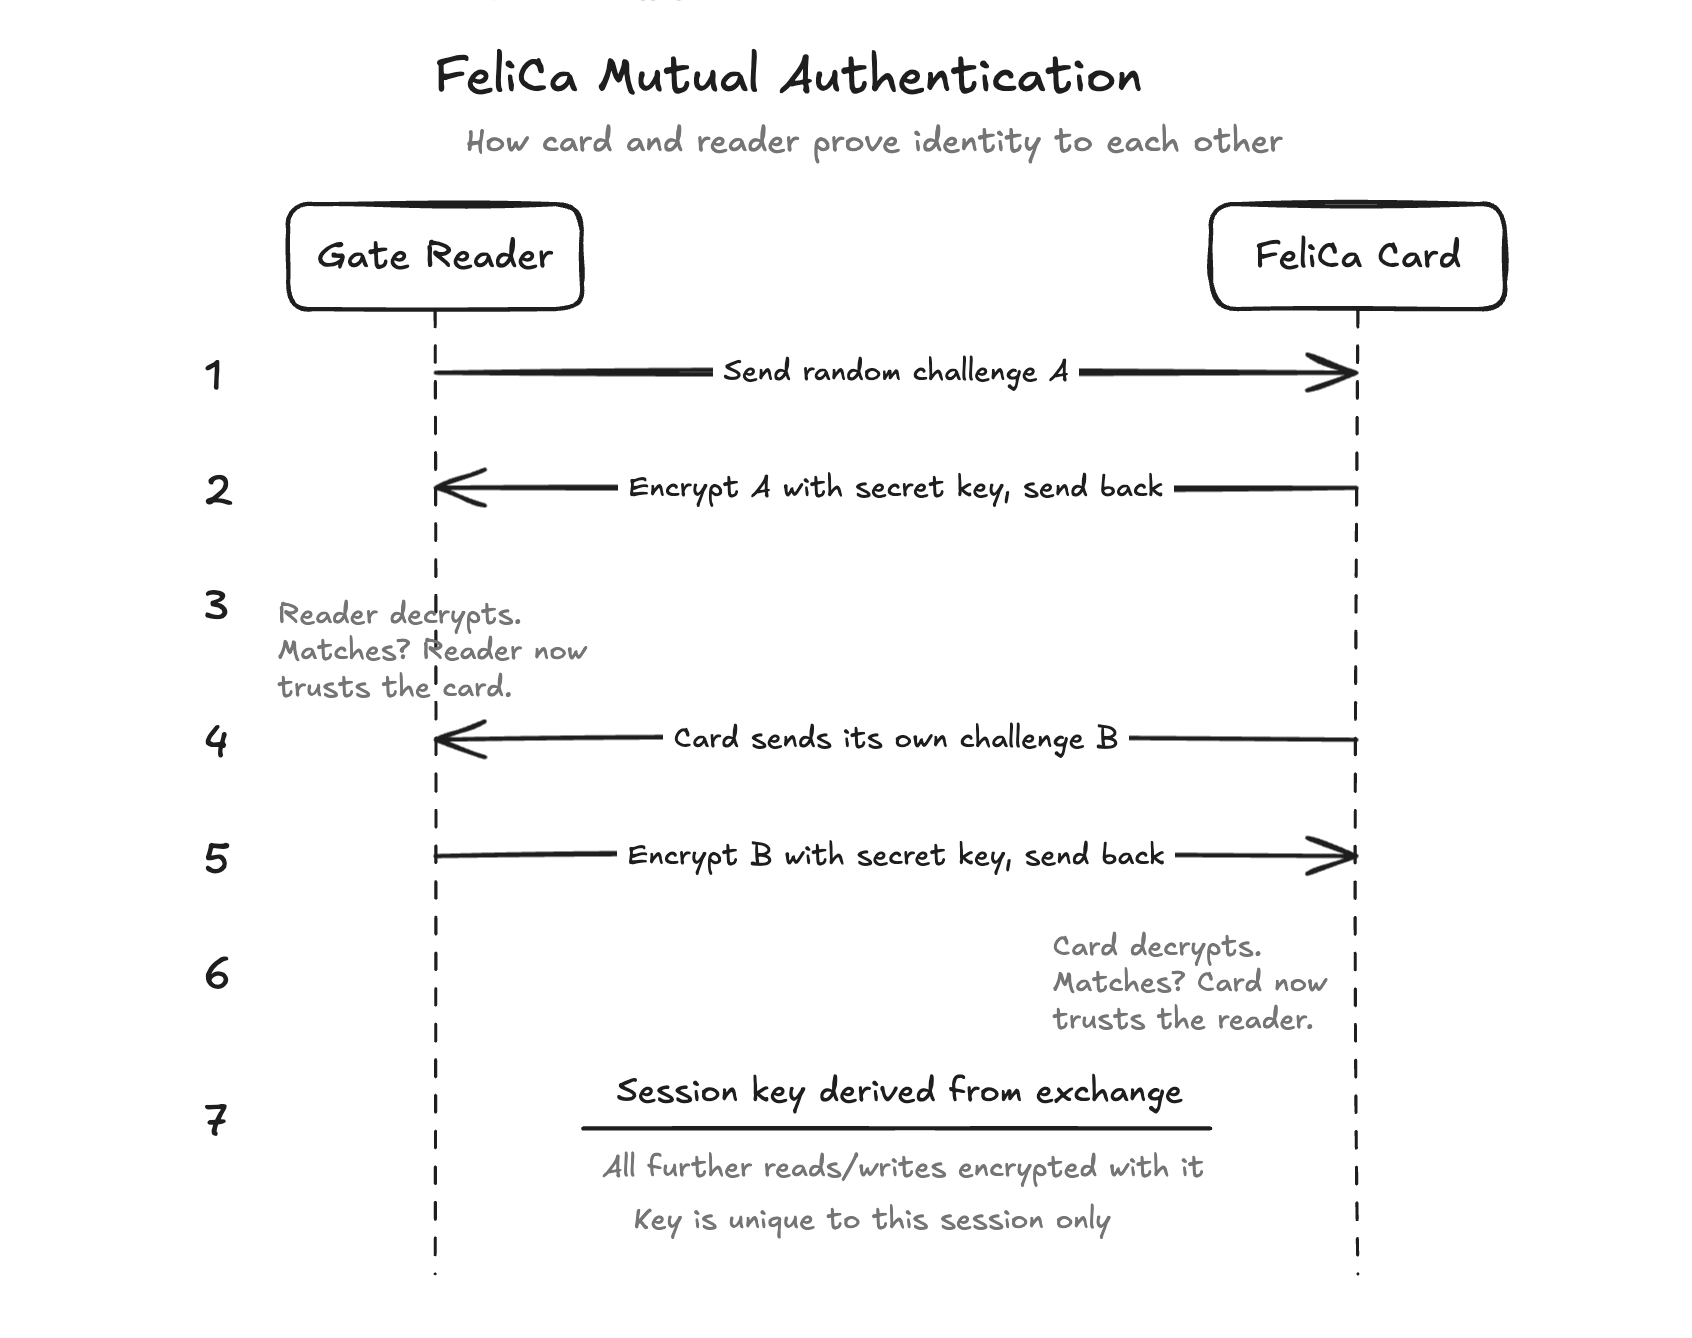
\includegraphics[width=0.85\textwidth]{images/felica-mutual-authentication.png}
    \caption{FeliCa mutual authentication flow between the gate reader and the contactless card. A new encryption key is derived for each session, making captured data useless for future transactions.}
    \label{fig:felica-auth}
\end{figure}

The way mutual authentication works is basically a challenge-response protocol. The reader generates a random number and sends it to the card as a challenge. The card takes that number, encrypts it with the secret key that is stored inside the chip, and sends the encrypted result back. The reader already knows the key too, so it can check if the response is correct. If it is, the reader knows it is talking to a legitimate card and not a fake one. Then the process goes the other way around: the card sends its own random challenge to the reader, the reader encrypts it with the same key, and the card checks the response. Only after both sides have verified each other does the actual balance read and write happen. At the end of this exchange, both sides derive a session key that is used to encrypt everything that follows. This session key is unique to this one transaction and will never be reused.

This design also makes card cloning very hard to pull off. The secret key lives inside the chip's secure memory and it never leaves it. You cannot read it out, not even if you physically open the card. So even if someone has a reader and captures all the radio signals during a transaction, the encrypted responses they capture are useless for next time because the challenges will be different. To fake a valid response, an attacker would need the actual secret key, and there is no way to get it from the captured data alone. What about physical attacks, like putting the chip under a microscope and probing the circuits, or doing power analysis where you measure the chip's electricity consumption to try to figure out the key? That is exactly what the EAL6+ certification covers. To get that certification level, the chip has to be tested against these kinds of hardware attacks and prove it can resist them.

Octopus in Hong Kong follows a similar model but expanded the use case beyond transit. Launched in September 1997, it was actually the first contactless smart card system in the world to adopt Sony's FeliCa technology~\cite{SonyOctopus}, four years before Suica. What started as a pure transit card evolved into a general-purpose stored-value card accepted at convenience stores, restaurants, parking garages, and even vending machines. By the early 2000s, it had over 11 million cards in circulation in a city of 7 million people, which gives you an idea of how widely adopted it became. The interesting thing about Octopus from our perspective is that it demonstrated that a closed-loop, card-stored-balance system could scale beyond its original domain while maintaining fast transaction times.

Now, what can we learn from these systems for our festival payment architecture? The first lesson is that speed matters a lot. Transit systems proved that sub-second transactions are not just nice to have, they are a hard requirement when you are processing large volumes of people who do not want to wait. At a festival, the same principle applies: nobody wants to stand in line for two minutes waiting for a payment to go through when they just want a beer.

The second lesson is about where the balance lives. Transit cards store the balance on the card chip, which is what makes offline operation possible. In a festival context, NFC bracelets can work in a similar way: the balance is written directly to the chip on the bracelet, and the vendor terminal reads and updates it locally, just like a Suica gate does with a FeliCa card. This means transactions can happen even without network connectivity. However, in our system we also support a smartphone app as an alternative to bracelets. With a phone, we cannot write balances directly to the NFC chip the way you can with a bracelet or a transit card. So for the app-based flow, the authoritative balance lives on the server, and during offline periods, vendor terminals work with cached snapshots of recent balances. This dual approach, bracelets with on-chip balances and phones with server-side balances, introduces its own set of challenges, which we will discuss in detail in Chapter~\ref{chap:architecture}.

The third lesson is about the limitations of the transit model. Transit systems operate in a very controlled environment: the terminals are fixed, maintained by professionals, connected to a private network, and the usage patterns are more or less predictable. A festival is a completely different story. Vendor terminals are mobile devices carried by staff who may not be very technical, the network is a temporary Wi-Fi setup in a field, and usage spikes happen unpredictably during meal breaks or between performances. So while transit systems show that offline closed-loop payments can work, their specific solutions do not transfer directly to our context.

\subsection{Festival Payment Systems}
\label{subsec:campus-cards}

Over the past decade, a whole industry has grown up around providing cashless payment solutions for festivals and events. Companies like Tappit, Intellitix, Weezevent, and Glownet have deployed their systems at hundreds of events worldwide. The typical setup works like this: attendees receive an RFID wristband when they enter the festival. They load credits onto the wristband using cash top-up stations or an online portal before the event. At each vendor point, there is a handheld terminal that reads the wristband, deducts the purchase amount, and writes the new balance back to the chip. It is essentially the same model as transit cards, adapted for the festival context.

These systems have proven that cashless festivals are commercially viable. As mentioned in Chapter~\ref{chap:introduction}, Tappit reports that RFID systems reduce transaction times by up to 80 percent compared to cash and increase average spending by about 22 percent~\cite{Tappit2024}. The speed improvement comes from eliminating the need to count cash and make change. The spending increase is attributed to the psychological effect of not physically handing over money, which is consistent with the broader academic literature on cashless payment behavior~\cite{Schomburgk2024}.

However, there are some significant limitations to the RFID wristband approach that motivated us to explore a different path. First, the RFID chips used in most festival wristbands have very limited storage and processing capability. They can store a balance and maybe a transaction counter, but they cannot run complex logic. This means that all the intelligence has to be in the terminal, and the terminal needs to handle things like transaction validation, balance updates, and security checks. If the terminal loses connectivity to the backend and its local cache is stale or incomplete, it has a problem.

Second, and this is the bigger issue, many of these RFID systems rely on MIFARE Classic chips, which have well-documented security vulnerabilities. Garcia et al.~\cite{Garcia2008} demonstrated practical attacks against MIFARE Classic's proprietary CRYPTO1 cipher, showing that the encryption could be broken and the card contents cloned or modified. For a payment system, this is a serious problem because it means that a sufficiently motivated attacker could tamper with their balance. More modern chips like MIFARE DESFire have addressed these vulnerabilities, but they are more expensive, and many festival deployments still use the older technology to keep costs down.

Third, the architectures of these commercial systems are proprietary and essentially undocumented. There is no published academic analysis of how Tappit or Intellitix handle offline operation, conflict resolution, or balance reconciliation. This makes it hard to learn from their design decisions or to identify best practices. All we have are the occasional failure reports, like the Download Festival incident mentioned in Chapter~\ref{chap:introduction}, which tell us what went wrong but not how things were supposed to work.

Since there is not a lot of published research on how these systems work in practice, we talked to people who were involved in deploying payment infrastructure at Untold, one of the largest music festivals in Romania. From those conversations we learned that the typical approach is to deploy a local network on-site and bring dedicated servers to the venue, so that the core payment logic runs locally and does not depend on a remote cloud. Even with this setup though, the network is still unreliable enough that top-up operations can take two to four hours to synchronize across all terminals when the Wi-Fi coverage gets bad. This is a real problem for attendees who just loaded money and want to spend it immediately but the vendor terminal does not know about it yet. It shows that maintaining reliable Wi-Fi coverage is not just something nice to have, it is a core infrastructure requirement for any festival payment system. We discuss how our architecture handles these synchronization delays in Chapter~\ref{chap:architecture}.

Given these trade-offs, there are two main directions we could take. One option is to stick with the RFID wristband model and use NFC bracelets with on-chip balances, which gives us the advantage of fully offline transactions like transit cards but limits what we can do on the user side. The other option is to go with a smartphone app as the consumer device, where the balance lives on the server and payments happen via QR codes or NFC between the phone and the vendor terminal. A phone-based approach gives more flexibility for things like showing transaction history, doing top-ups from the app, and pushing notifications, but it means we depend more on the network since the balance is not stored locally on a chip. There is also a middle ground where we support both. We explore these options further in Chapter~\ref{chap:architecture}.

\subsection{EMV and Offline Authorization}
\label{subsec:emv}

The EMV standard, named after its original creators Europay, Mastercard, and Visa, is the technology behind the chip cards that most people carry in their wallets. While EMV is an open-loop standard designed for the global payment network, it includes a mechanism for offline transaction authorization that is worth understanding because it addresses a similar problem to ours: how do you authorize a payment when you cannot reach the authorization server?

The way EMV offline authorization works is through a set of risk parameters stored on the card chip. The card knows its own balance limits, the maximum amount for a single offline transaction, the maximum number of offline transactions allowed before the card must go online, and the total cumulative amount that can be spent offline. When a merchant terminal cannot reach the bank's authorization server, it can still approve transactions by checking these parameters locally. If the transaction falls within the allowed limits, it gets approved offline. If it exceeds them, the terminal declines the transaction or forces an online authorization attempt.

This is a clever approach because it distributes the risk. The card issuer decides how much offline risk they are willing to accept for each cardholder, and those limits are baked into the card at the time of issuance. A premium cardholder might have higher offline limits than a basic cardholder. The merchant also has some say in this: their terminal can have its own floor limit below which it will always accept transactions without going online.

However, there is a well-known problem with EMV offline authorization: the system trusts the card to honestly report its own state. Murdoch et al.~\cite{Murdoch2010} demonstrated a man-in-the-middle attack on the EMV protocol where a device placed between the card and the terminal could trick the terminal into believing that a PIN had been correctly verified when it had not. While this specific attack targets the PIN verification rather than the offline balance logic, it illustrates a broader point: any system where the authorization decision depends on data stored on a device in the user's possession is vulnerable to tampering if the security of that device is compromised.

For our system, the EMV offline model offers both inspiration and a warning. On the inspiration side, the idea of using spending limits to control offline risk is directly applicable. We implement something similar: during offline periods, vendor terminals enforce a maximum transaction amount and a maximum total offline spend per consumer, which limits the potential damage from double-spending or stale balance snapshots. On the warning side, the EMV experience shows that offline authorization always involves a trade-off between availability and security. The more you allow offline, the more risk you accept. Our system handles this by keeping offline periods as short as possible and treating offline mode as a temporary fallback rather than a primary operating mode.

\section{Offline-First Architecture Patterns}
\label{sec:offline-first}

When you build a system that needs to work without a network connection, you are basically deciding where on a spectrum your application sits. On one end you have fully online systems, where every operation needs a round-trip to a server and nothing works without internet. On the other end you have fully offline systems, like the FeliCa transit cards we discussed earlier, where everything happens locally and the network is only used for background synchronization. Most real-world applications fall somewhere in between.

For our festival payment system, we need to be somewhere in the middle of this spectrum. The system should work online by default, because that gives us the strongest guarantees about balance correctness and transaction ordering. But when the network goes down, and at a festival it will go down, the system needs to keep processing payments using whatever data it has cached locally. This means we need architectural patterns that support both modes of operation and can switch between them without losing data or creating inconsistencies that cannot be resolved later.

In this section we look at four architectural patterns that are relevant to this problem. Each one addresses a different aspect of building systems that can work without constant connectivity.

\subsection{Local-First Software}
\label{subsec:local-first}

The term ``local-first software'' was introduced by Kleppmann et al.~\cite{Kleppmann2019} in a 2019 paper that argued for a different way of thinking about where data lives in an application. The basic idea is that the primary copy of the data should be on the user's local device, not on a remote server. The cloud still exists, but its role is to sync data between devices rather than to be the single source of truth. If the server goes down, or the network disappears, the application keeps working because the data is right there on the device.

Kleppmann and his co-authors defined seven ideals for local-first software: no spinners (the app should be fast because it reads from local storage), the user's work should be available on multiple devices, the network should be optional, collaboration should be seamless, the data should be accessible for a long time (not locked behind a service that might shut down), security and privacy should be built in, and the user should have full ownership and control over their data.

Now, our festival payment system does not fit neatly into the local-first model, and there is a good reason for that. In a collaborative document editor, if two people edit the same paragraph and the results get merged a bit awkwardly, that is annoying but not catastrophic. In a payment system, if two terminals both think a user has 50 euros and each one authorizes a 40 euro purchase, you have just lost 30 euros. Money is a conserved quantity. You cannot merge two versions of a balance the way you merge two versions of a text document.

That said, some of the local-first principles are directly useful for us. The idea of keeping a local copy of the data so the app does not freeze when the network drops is exactly what our vendor terminals need to do. The difference is that in our case, the local copy is a read cache with limited write authority, not the primary copy. The server remains the source of truth, and offline transactions are treated as provisional until they get confirmed by the server. This is a weaker version of local-first, but it is the right trade-off for a system where financial correctness matters more than collaboration flexibility.

\subsection{Conflict-Free Replicated Data Types (CRDTs)}
\label{subsec:crdts}

CRDTs, or Conflict-Free Replicated Data Types, are data structures specifically designed for systems where multiple nodes can modify the same data independently, without coordinating with each other, and still end up in a consistent state. They were formalized by Shapiro et al.~\cite{Shapiro2011} in 2011, and the key property that makes them work is that all operations on the data structure are designed to be commutative, associative, and idempotent. What this means in practice is that it does not matter what order the updates arrive in, or if some updates arrive more than once. The result will always be the same.

The simplest example is a G-Counter (grow-only counter). Imagine you have five terminals at a festival, and each one counts how many transactions it has processed. Each terminal only increments its own counter. When they sync, you just take the maximum value for each terminal's counter and sum them up. No conflicts possible. A PN-Counter extends this idea by having two G-Counters, one for increments and one for decrements, and the actual value is the difference between the two.

This sounds like it could work for tracking balances, but there is a catch. A balance is not just a counter that goes up and down freely. Money is conserved: you cannot spend more than you have. CRDTs are great at ensuring convergence (everyone ends up with the same value), but they do not enforce invariants like ``the balance must not go below zero.'' If two terminals independently authorize purchases against the same balance while offline, a naive CRDT approach would let both go through, even if the total exceeds the available balance. You would only discover the overspend after synchronization.

Kleppmann~\cite{Kleppmann2017json} explored this limitation in the context of JSON CRDTs and noted that while CRDTs guarantee convergence, they do not guarantee that the converged state is one that any individual node would have accepted. For payment systems, this is a real problem. We cannot just let every offline transaction go through and hope the math works out later.

So for a payment system, pure CRDTs are not enough on their own. You need something extra on top to deal with the fact that balances have constraints. There are a few ways to handle this. One option is to record offline transactions as events and have the server replay and validate them when connectivity returns, rejecting any that would overdraw the balance. Another option is to pre-allocate spending limits per terminal so that each terminal can only authorize up to a fixed amount while offline, which reduces the chance of overspending in the first place. A third option is some combination of the two. We explore these trade-offs further in Chapter~\ref{chap:architecture}.

\subsection{Event Sourcing and CQRS}
\label{subsec:event-sourcing}

Event sourcing is a pattern where instead of storing the current state of an object (like ``balance = 47.50''), you store the entire sequence of events that led to that state (``topped up 50.00, bought beer for 2.50''). The current state can always be reconstructed by replaying the events from the beginning. Fowler~\cite{Fowler2005} describes event sourcing as a way to ``ensure that all changes to application state are stored as a sequence of events,'' and one of the main benefits is that you get a complete audit trail for free.

This pattern fits really well with offline payment processing. When a vendor terminal goes offline, it cannot update the central database directly. But it can keep recording events locally: ``user X paid 5.00 for item Y at timestamp Z.'' Each event is self-contained and immutable. When the terminal reconnects, it uploads its event log to the server, and the server can process these events in order to update the authoritative state. If there is a conflict (say, the user ran out of money between two offline purchases), the server can detect it during replay and handle it according to whatever policy the operator has defined.

CQRS, which stands for Command Query Responsibility Segregation, is a related pattern that is often used together with event sourcing. The idea, as described by Young~\cite{Young2010}, is to separate the write side of the system (commands that modify state) from the read side (queries that return data). In a traditional system, the same data model handles both reads and writes. In CQRS, you have one model optimized for processing writes (accepting payment events) and another model optimized for fast reads (showing the current balance on a screen).

For our system, this separation is useful because the write side and the read side have very different requirements. On the write side, we need strong ordering guarantees and conflict detection. On the read side, vendor terminals need to quickly look up a user's balance to decide whether to authorize a payment, and this lookup needs to work even when the terminal is offline. By separating these concerns, we can have the read model work from a local cache while the write model queues events for later synchronization, without the two getting in each other's way.

\subsection{Edge Computing}
\label{subsec:edge-computing}

Edge computing is the idea of moving computation closer to where the data is generated, instead of sending everything to a central server or cloud for processing. Shi et al.~\cite{Shi2016} describe it as ``pushing the frontier of computing applications, data, and services away from centralized nodes to the logical extremes of a network.'' In practice, this means doing as much work as possible on the device that is closest to the user, and only involving the cloud when necessary.

In the context of our festival payment system, the vendor terminals are the edge nodes. Each terminal runs a local instance of the payment logic: it can read a user's balance from its local cache, validate a transaction against the cached data, record the transaction as an event, and update its local view of the balance. All of this happens on the terminal itself without any network communication. The cloud server (or the on-site local server, as we discussed in the context of the Untold festival) acts as the central coordinator that collects events from all the edge nodes, resolves conflicts, and pushes updated state back out.

This works well for festival environments because the network is the weakest link in the whole system. The less you depend on it for individual transactions, the better. If the terminal can handle a payment entirely on its own, then a network outage does not mean a payment outage. It just means that the synchronization of data gets delayed. The trade-off, of course, is that edge nodes are working with potentially stale data. A terminal that has been offline for 30 minutes might not know about a top-up that happened 20 minutes ago. How we handle this staleness, and what limits we put on edge-processed transactions to manage the risk, is something we cover in detail in Chapter~\ref{chap:architecture}.

\section{Conflict Resolution in Distributed Systems}
\label{sec:conflict-resolution}

When multiple vendor terminals at a festival are processing payments independently, without being able to talk to each other or to a central server, they are going to end up with different views of the world. Terminal A might think a user has 50 euros because it processed a top-up, while Terminal B still shows the old balance of 20 euros because it has not received the update yet. If both terminals authorize purchases during this window, the system will have conflicting records that need to be sorted out once everyone reconnects.

This is not a new problem. Distributed systems have been dealing with conflicting state for decades, and there is a solid body of theory and practice around how to handle it. In this section we go through the main concepts that are relevant to our case: what trade-offs are fundamental and cannot be avoided, how systems achieve consistency without requiring all nodes to agree in real-time, how to figure out the order of events when there is no shared clock, and how to let nodes work independently with the plan of fixing things up later.

\subsection{The CAP Theorem}
\label{subsec:cap-theorem}

In 2000, Eric Brewer presented a conjecture at the ACM Symposium on Principles of Distributed Computing that would become one of the most cited results in distributed systems. The conjecture, which Gilbert and Lynch~\cite{Gilbert2002} formally proved in 2002, says that a distributed system can only guarantee two out of three properties at the same time: Consistency (every node sees the same data at the same time), Availability (every request to a non-failing node gets a response), and Partition Tolerance (the system keeps working even when the network between nodes is broken).

The important word here is ``partition tolerance.'' In a festival environment, network partitions are not an edge case, they are a regular occurrence. When the Wi-Fi drops between two parts of the venue, the vendor terminals on each side are partitioned from each other and from the server. At that point, according to CAP, we have to choose: do we want consistency or availability?

If we choose consistency, then when a terminal cannot reach the server to verify a balance, it should refuse the transaction. The data stays consistent, but the system is unavailable and the attendee cannot buy anything. If we choose availability, the terminal goes ahead and authorizes the payment based on its local cache, even though it cannot be sure the data is up to date. The payment goes through, the attendee is happy, but we might end up with inconsistencies that have to be fixed later.

For a festival payment system, refusing transactions because the network is down is not really an option. Nobody is going to accept a system that stops working every time the Wi-Fi gets flaky, which at a festival is all the time. So during network partitions, our system leans toward availability. Transactions keep going through, and consistency is restored after the partition heals. This is not a unique choice. Many real-world systems choose availability during partitions and then run a reconciliation process afterward. That is essentially what we are doing.

\subsection{Eventual Consistency}
\label{subsec:eventual-consistency}

If we are giving up strong consistency during network partitions, the question becomes: what kind of consistency can we actually promise? The answer, for most distributed systems that prioritize availability, is eventual consistency. Vogels~\cite{Vogels2009} defines it simply: if no new updates are made to a piece of data, then eventually all replicas will converge to the same value.

The word ``eventually'' is doing a lot of work in that definition. It does not say when the replicas will agree, just that they will at some point. In practice, this usually happens pretty fast once connectivity is restored. But during the partition, different nodes can have different views of the data, and that is considered acceptable.

The most famous real-world example of eventual consistency is Amazon's Dynamo, described by DeCandia et al.~\cite{DeCandia2007}. Dynamo is a key-value store that Amazon built for their shopping cart and other services that need to be available all the time, even during failures. Dynamo allows writes to happen on any node, even if that node cannot reach the others. When the partition heals, Dynamo uses application-specific logic to merge conflicting versions.

For our system, eventual consistency means the following: while terminals are offline, they work with their local data and record all transactions locally. When they reconnect, they send their transaction logs to the server. The server processes everything, figures out the correct state of each balance, and pushes the updated data back to all terminals. At that point, everyone is consistent again. The window during which terminals might have stale or conflicting data is the offline period, and the goal of the architecture is to make this window as short as possible and to limit the damage that can happen during it (for example, by capping how much a terminal can authorize while offline).

\subsection{Transaction Ordering and Why Timestamps Are Enough}
\label{subsec:transaction-ordering}

One of the classic problems in distributed systems is figuring out the order in which things happened across different nodes. The standard solutions from the literature are logical clocks and vector clocks, which use counters instead of real time to establish ordering. These are necessary in systems like high-frequency trading platforms, where events happen microseconds apart on different machines and physical clock drift is larger than the interval between events.

However, for a festival payment system, the situation is fundamentally different. Transactions happen at human speed. A person walks to a vendor, waits in line, orders something, taps their wristband. The gap between one transaction and the next, even for the same user, is measured in minutes, not microseconds. Even cheap NTP synchronization keeps clocks within a few hundred milliseconds of each other, and that kind of drift is completely irrelevant when the events we care about are minutes apart.

This means that plain wall-clock timestamps, recorded by each vendor terminal at the moment of the transaction, give us unambiguous ordering in practice. There is no realistic scenario where two transactions from the same user happen so close together that clock drift changes the order. The physical constraint of the wristband model reinforces this: a user can only be at one vendor at a time, so transactions from the same user are naturally serialized by their physical presence.

The practical advantage of using timestamps over vector clocks is significant. With timestamps, vendor terminals do not need to communicate with each other at all during offline periods. Each terminal just records its local time with each transaction. When the network comes back, everyone pushes their logs to the server, the server sorts by timestamp, and we are done. There is no vector state to maintain, no counter synchronization between devices, and no extra complexity in the protocol. For a system that needs to work reliably in a festival environment where connectivity is unreliable, this simplicity is a real advantage.
